\documentclass[11pt]{article}
\usepackage[margin=1in]{geometry}
\usepackage{amsmath,amssymb,amsthm,mathtools,bm}
\usepackage{booktabs,array,tabularx}
\usepackage{tikz}
\usetikzlibrary{arrows.meta,decorations.markings,calc}
\usepackage[dvipsnames]{xcolor}
\usepackage{tcolorbox}
\usepackage[numbers,sort&compress]{natbib}
\usepackage[colorlinks=true,linkcolor=RoyalBlue,citecolor=ForestGreen,urlcolor=RoyalBlue]{hyperref}
\usepackage[capitalise]{cleveref}

% ---------- macros ----------
\newcommand{\Tr}{\operatorname{Tr}}
\newcommand{\Lc}{\mathcal{L}}
\newcommand{\Pc}{\mathcal{P}}
\newcommand{\Qc}{\mathcal{Q}}
\newcommand{\Kc}{\mathcal{K}}
\newcommand{\Gc}{\mathcal{G}}
\newcommand{\ee}{\mathrm{e}}
\newcommand{\dd}{\mathrm{d}}
\newcommand{\cl}{\mathrm{c}}
\newcommand{\qu}{\mathrm{q}}
\newcommand{\rhoS}{\rho_{S}}
\newcommand{\rhoB}{\rho_{B}}
\newcommand{\ket}[1]{|#1\rangle}
\newcommand{\bra}[1]{\langle#1|}
\newcommand{\avg}[1]{\langle#1\rangle}
\newcommand{\acomm}[2]{\{#1,#2\}}
\newcommand{\comm}[2]{[#1,#2]}

\newtcolorbox{keybox}[1][]{colback=RoyalBlue!4,colframe=RoyalBlue!60,
  fonttitle=\bfseries,title={#1},boxrule=0.6pt,arc=2pt,left=4pt,right=4pt,top=3pt,bottom=3pt}
\newtcolorbox{warnbox}{colback=Orange!6,colframe=Orange!70,boxrule=0.6pt,arc=2pt,
  left=4pt,right=4pt,top=3pt,bottom=3pt}

\newtheorem{exercise}{Exercise}

\title{\textbf{Keldysh and Mori--Zwanzig}\\[2pt]
\large Two languages for the same open-system dynamics:\\ a working note and a self-study plan\\[4pt] \normalsize Version 2}
\author{Notes prepared with Claude}
\date{15 October 2026 (v2; v1: 30 September 2026)}

\begin{document}
\maketitle

\begin{warnbox}
\small\textbf{About the references.} All bibliography entries were checked on
30~September~2026 against publisher, Crossref, or arXiv records, and DOIs were added
where they exist. The equations in the main text were derived and cross-checked
independently of the references.\\[3pt]\textbf{Changes in v2.} \Cref{sec:keldysh-rho} was rewritten and expanded: it now derives the contour from the second-order term of $U\rho U^\dagger$, works out the Keldysh rotation on a qubit, derives the $2\times2$ (Larkin--Ovchinnikov) structure of the bath contractions from the $\pm$ basis, checks the second-order and fourth-order diagrams explicitly, and derives the influence functional as the commutative limit of the Wick sum. Equation numbers after \cref{sec:keldysh-rho} have shifted; labels are unchanged.
\end{warnbox}

\begin{keybox}[The thesis in three lines]
\begin{enumerate}\itemsep0pt
\item \emph{Density-matrix level.} Ordering Liouville-space superoperators along a
  single real time axis \emph{is} Keldysh contour ordering. With the Nakajima projector
  $\Pc=\rhoB\otimes\Tr_B$ and a Gaussian bath, the NZ memory kernel is the
  \emph{irreducible self-energy} of the reduced propagator, and the NZ equation is a
  Dyson equation.
\item \emph{Operator level.} Mori's projection onto a system operator $A$ yields a
  generalized Langevin equation. For $A=c$ with the anticommutator inner product, the
  Mori memory function is (up to a factor $-i$) the \emph{retarded} self-energy
  $\Sigma^R$.
\item \emph{Common ground.} Both expansions are built from the two bath kernels that
  appear in the Keldysh/Feynman--Vernon influence functional: the response
  $\chi$ (retarded, $\mathrm{c}\text{--}\mathrm{q}$) and the noise $S$ (Keldysh,
  $\mathrm{c}\text{--}\mathrm{c}$). Differences between the methods come from
  \emph{which object is projected} and \emph{how the series is resummed}, not from
  different physics.
\end{enumerate}
\end{keybox}

\tableofcontents

%=====================================================================
\section{Setup and conventions}
\label{sec:setup}

We set $\hbar=1$ throughout and take
\begin{equation}
  H = H_S + H_B + H_I,\qquad H_I=\sum_\alpha S_\alpha\otimes B_\alpha ,
\end{equation}
with Hermitian $S_\alpha$, $B_\alpha$, a stationary bath state $\rhoB$ ($[H_B,\rhoB]=0$),
and $\avg{B_\alpha}\equiv\Tr_B(B_\alpha\rhoB)=0$. The Liouvillian is
$\Lc X=-i[H,X]=(\Lc_S+\Lc_B+\Lc_I)X$. For a factorized initial state
$\rho(0)=\rhoS(0)\otimes\rhoB$, the reduced dynamics defines the dynamical map
\begin{equation}
  \rhoS(t)=\Pi(t)\,\rhoS(0),\qquad \Pi(t)X\equiv\Tr_B\!\big[\ee^{\Lc t}(X\otimes\rhoB)\big].
  \label{eq:map}
\end{equation}

\paragraph{Left/right superoperators and the Keldysh rotation.}
For any operator $A$, define $A^{+}X=AX$ (acting on the ket, i.e.\ the \emph{forward}
branch) and $A^{-}X=XA$ (acting on the bra, i.e.\ the \emph{backward} branch). Then
$\Lc_I=-i(H_I^{+}-H_I^{-})$. The Keldysh rotation to ``classical'' and ``quantum''
combinations is
\begin{equation}
  A^{\cl}=\tfrac12\big(A^{+}+A^{-}\big)\;\;\big(A^{\cl}X=\tfrac12\{A,X\}\big),\qquad
  A^{\qu}=A^{+}-A^{-}\;\;\big(A^{\qu}X=[A,X]\big).
  \label{eq:rotation}
\end{equation}
Since system and bath superoperators commute,
$S^+B^+-S^-B^-=S^{\cl}B^{\qu}+S^{\qu}B^{\cl}$, and therefore
\begin{equation}
  \boxed{\;\Lc_I=-i\sum_\alpha\big(S^{\qu}_\alpha B^{\cl}_\alpha+S^{\cl}_\alpha B^{\qu}_\alpha\big).\;}
  \label{eq:LIcq}
\end{equation}
Two trace identities do most of the work: $\Tr_B(B^{\qu}Y)=0$ for any $Y$ (the trace of a
commutator vanishes), and $\Tr_B(B^{\cl}Y)=\Tr_B(BY)$.

\paragraph{Bath kernels.}
With $B_\alpha(t)=\ee^{iH_Bt}B_\alpha\ee^{-iH_Bt}$,
\begin{align}
  S_{\alpha\beta}(t)&=\tfrac12\avg{\{B_\alpha(t),B_\beta(0)\}}
  &&\text{(symmetrized noise; Keldysh component)},\\
  \chi_{\alpha\beta}(t)&=i\,\theta(t)\avg{[B_\alpha(t),B_\beta(0)]}
  &&\text{(Kubo response; retarded component)}.
\end{align}
The full correlator is $C_{\alpha\beta}(t)=\avg{B_\alpha(t)B_\beta}=S_{\alpha\beta}(t)-\tfrac{i}{2}\chi_{\alpha\beta}(t)$
for $t>0$. For a single Hermitian $B$, $S(t)$ is real and even. In thermal equilibrium the
fluctuation--dissipation theorem (FDT) reads $S(\omega)=\coth(\beta\omega/2)\,\chi''(\omega)$, with
$S(\omega)=\int\!\dd t\,\ee^{i\omega t}S(t)$ and $\chi''=\operatorname{Im}\chi$. Up to factors of $i$, these are the bath
Green's functions $D^K$ and $D^R$ of Keldysh field theory~\cite{Kamenev2011,KamenevLevchenko2009}.

%=====================================================================
\section{Keldysh on the density matrix: why the contour is already there}
\label{sec:keldysh-rho}

The claim of this section is that nothing has to be \emph{added} to the von Neumann
equation to obtain the Keldysh contour. The contour, the $\cl/\qu$ rotation, the
$2\times2$ matrix structure of the bath propagator and the causality rules all appear
on their own once one treats $\rho$ as a vector and $H$ as a pair of superoperators.
We go through this slowly, with one worked example for each step. The results that the
rest of the note depends on are \cref{eq:contractions} (the contractions) and
\cref{eq:FV} (the influence functional); the intermediate steps are there to make
those two formulas feel inevitable.

\begin{figure}[t]
\centering
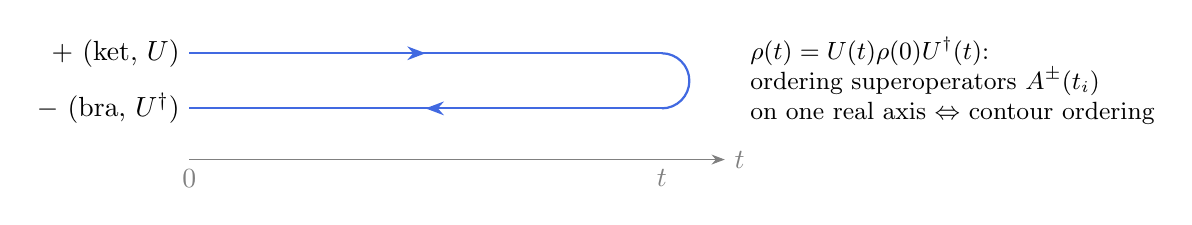
\begin{tikzpicture}[>=Stealth,scale=1.0]
  % contour
  \draw[thick,RoyalBlue,postaction={decorate},decoration={markings,mark=at position 0.5 with {\arrow{>}}}]
      (0,0.35) -- (6,0.35);
  \draw[thick,RoyalBlue] (6,0.35) arc (90:-90:0.35);
  \draw[thick,RoyalBlue,postaction={decorate},decoration={markings,mark=at position 0.5 with {\arrow{>}}}]
      (6,-0.35) -- (0,-0.35);
  \node[left] at (0,0.35) {$+$ (ket, $U$)};
  \node[left] at (0,-0.35) {$-$ (bra, $U^\dagger$)};
  \draw[->,gray] (0,-1.0) -- (6.8,-1.0) node[right] {$t$};
  \node[below,gray] at (0,-1.0) {$0$};
  \node[below,gray] at (6,-1.0) {$t$};
  \node[right,align=left,font=\small] at (7.0,0.0) {$\rho(t)=U(t)\rho(0)U^\dagger(t)$:\\
  ordering superoperators $A^\pm(t_i)$\\ on one real axis $\Leftrightarrow$ contour ordering};
\end{tikzpicture}

\vspace{6pt}
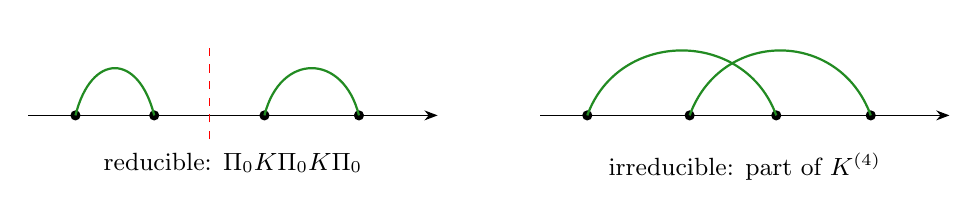
\begin{tikzpicture}[>=Stealth,scale=1.0]
  \tikzset{v/.style={circle,fill=black,inner sep=1.3pt}}
  % reducible
  \draw[->] (0,0)--(5.2,0);
  \foreach \x in {0.6,1.6,3.0,4.2} \node[v] at (\x,0) {};
  \draw[thick,ForestGreen] (0.6,0) .. controls (0.8,0.8) and (1.4,0.8) .. (1.6,0);
  \draw[thick,ForestGreen] (3.0,0) .. controls (3.2,0.8) and (4.0,0.8) .. (4.2,0);
  \draw[dashed,red] (2.3,-0.3)--(2.3,0.9);
  \node[below,font=\small] at (2.6,-0.35) {reducible: $\Pi_0K\Pi_0K\Pi_0$};
  % irreducible
  \begin{scope}[xshift=6.5cm]
  \draw[->] (0,0)--(5.2,0);
  \foreach \x in {0.6,1.9,3.0,4.2} \node[v] at (\x,0) {};
  \draw[thick,ForestGreen] (0.6,0) .. controls (1.0,1.1) and (2.6,1.1) .. (3.0,0);
  \draw[thick,ForestGreen] (1.9,0) .. controls (2.3,1.1) and (3.8,1.1) .. (4.2,0);
  \node[below,font=\small] at (2.6,-0.35) {irreducible: part of $K^{(4)}$};
  \end{scope}
\end{tikzpicture}
\caption{Top: the Keldysh contour. The forward and backward branches are the ket and
bra sides of $\rho$. Bottom: real-time diagrams for the reduced propagator. Vertices are
system superoperators $S^{\cl/\qu}$ and lines are bath contractions ($S$ or $\chi$). A
diagram that can be cut between vertices without cutting a line (red) is reducible. The
NZ kernel collects exactly the irreducible diagrams.}
\label{fig:contour}
\end{figure}

%---------------------------------------------------------------------
\subsection{The contour from the von Neumann equation}
\label{sec:contour-from-vN}

Work in the interaction picture with respect to $H_0=H_S+H_B$, so that
$\tilde H_I(t)=\ee^{iH_0t}H_I\ee^{-iH_0t}$ and $\tilde\rho(t)=\tilde U(t)\rho(0)\tilde U^\dagger(t)$ with
\begin{equation}
  \tilde U(t)=T\exp\Big[-i\!\int_0^t\!\dd s\,\tilde H_I(s)\Big]
  =1-i\!\int_0^t\!\dd t_1\tilde H_I(t_1)-\!\int_0^t\!\dd t_1\!\int_0^{t_1}\!\dd t_2\,\tilde H_I(t_1)\tilde H_I(t_2)+\dots
\end{equation}
Its adjoint is \emph{anti}-time-ordered: in $\tilde U^\dagger$ the later operator stands to
the right, $\tilde U^\dagger=1+i\int\tilde H_I-\int_{t_1>t_2}\tilde H_I(t_2)\tilde H_I(t_1)+\dots$

\begin{keybox}[Example: the second-order term, written out]
Collecting all terms of order $H_I^2$ in $\tilde U\rho(0)\tilde U^\dagger$,
\begin{align}
  \tilde\rho^{(2)}(t)=&-\int_0^t\!\dd t_1\!\int_0^{t_1}\!\dd t_2\,\tilde H_I(t_1)\tilde H_I(t_2)\,\rho(0)
   &&\text{(both on the ket side; time-ordered)}\notag\\
  &-\int_0^t\!\dd t_1\!\int_0^{t_1}\!\dd t_2\,\rho(0)\,\tilde H_I(t_2)\tilde H_I(t_1)
   &&\text{(both on the bra side; anti-time-ordered)}\notag\\
  &+\int_0^t\!\dd t_1\!\int_0^{t}\!\dd t_2\,\tilde H_I(t_1)\,\rho(0)\,\tilde H_I(t_2)
   &&\text{(one on each side; \emph{no} mutual ordering)}.
  \label{eq:rho2}
\end{align}
The third term is the one that looks unusual: $t_1$ and $t_2$ are integrated
independently over $[0,t]$, so there is no time ordering between a ket-side and a
bra-side operator. All three terms become a \emph{single} ordering rule once we say that
every point on the forward ($+$) branch is ``earlier'' than every point on the backward
($-$) branch, that time runs forward on $+$ and backward on $-$, and that operators are
ordered with later contour positions to the \emph{left} of $\rho(0)$ or to the \emph{right}
of it according to their branch. That rule is contour ordering, \cref{fig:contour}
(top)~\cite{Schwinger1961,Keldysh1964}.
\end{keybox}

The superoperator language makes the rule automatic. With $A^{+}X=AX$ and $A^{-}X=XA$,
\begin{equation}
  \tilde\rho^{(2)}(t)=\int_0^t\!\dd t_1\!\int_0^{t_1}\!\dd t_2\,
  \tilde\Lc_I(t_1)\tilde\Lc_I(t_2)\,\rho(0),\qquad
  \tilde\Lc_I(s)=-i\big[\tilde H_I^{+}(s)-\tilde H_I^{-}(s)\big],
  \label{eq:rho2super}
\end{equation}
and multiplying out the two brackets reproduces the three terms of \cref{eq:rho2}:
$H^+H^+$ gives the first, $H^-H^-$ gives the second (note $H^-(t_1)H^-(t_2)\rho=\rho H(t_2)H(t_1)$,
automatically anti-ordered), and the cross terms $H^+(t_1)H^-(t_2)+H^-(t_1)H^+(t_2)$ give
$H(t_1)\rho H(t_2)+H(t_2)\rho H(t_1)$ restricted to $t_1>t_2$, which is the third term with
its two orderings separated. In other words,
\begin{keybox}[Statement]
Ordinary time ordering of the superoperators $\tilde\Lc_I(t_i)$ along the single real axis
$[0,t]$, with a sum over the branch index $\pm$ at each vertex, \emph{is} Keldysh contour
ordering. One never has to think about the contour again: it is encoded in the sign of
$\Lc_I$ and the left/right action of $H^\pm$.
\end{keybox}

%---------------------------------------------------------------------
\subsection{The Keldysh rotation in Liouville space}
\label{sec:rotation-liouville}

The $\pm$ basis is natural for deriving the contour but awkward for calculations, because
the two branches are strongly correlated (the trace at the final time glues them
together). The Keldysh rotation \eqref{eq:rotation} separates ``what the two branches
have in common'' ($\cl$) from ``how they differ'' ($\qu$). Inverting it,
\begin{equation}
  A^{+}=A^{\cl}+\tfrac12A^{\qu},\qquad A^{-}=A^{\cl}-\tfrac12A^{\qu}.
  \label{eq:rotation-inverse}
\end{equation}

\paragraph{Derivation of \cref{eq:LIcq}.}
Since $S$ and $B$ act on different factors of the Hilbert space, $S^\pm$ and $B^\pm$ commute and
$(SB)^\pm=S^\pm B^\pm$. Then with \cref{eq:rotation-inverse},
\begin{align}
  S^{+}B^{+}-S^{-}B^{-}
  &=\big(S^\cl+\tfrac12S^\qu\big)\big(B^\cl+\tfrac12B^\qu\big)
   -\big(S^\cl-\tfrac12S^\qu\big)\big(B^\cl-\tfrac12B^\qu\big)\notag\\
  &=S^\cl B^\qu+S^\qu B^\cl ,
\end{align}
the $S^\cl B^\cl$ and $\frac14S^\qu B^\qu$ terms cancelling. Hence
$\Lc_I=-i\sum_\alpha(S^\qu_\alpha B^\cl_\alpha+S^\cl_\alpha B^\qu_\alpha)$, which is
\cref{eq:LIcq}. The structure ``one $\cl$, one $\qu$ per vertex'' is the same as in the
Keldysh action, where the interaction term $H_+-H_-$ is odd in the quantum field and so
always contains at least one $\qu$ leg.

\paragraph{What $\cl$ and $\qu$ do to a density matrix.}
It helps to see the two superoperators act on something concrete.

\begin{keybox}[Example: $\sigma_z^\cl$ and $\sigma_z^\qu$ on a qubit]
Write $\rho=\sum_{ij}\rho_{ij}\ket i\bra j$ with $\sigma_z\ket i=z_i\ket i$, $z_0=+1$, $z_1=-1$. Then
\begin{equation}
  \sigma_z^\cl\,\ket i\bra j=\tfrac12\{\sigma_z,\ket i\bra j\}=\tfrac{z_i+z_j}{2}\ket i\bra j,\qquad
  \sigma_z^\qu\,\ket i\bra j=[\sigma_z,\ket i\bra j]=(z_i-z_j)\ket i\bra j .
\end{equation}
In the Liouville basis $(\ket0\bra0,\ket0\bra1,\ket1\bra0,\ket1\bra1)$ both are diagonal:
\begin{equation}
  \sigma_z^\cl=\operatorname{diag}(1,0,0,-1),\qquad
  \sigma_z^\qu=\operatorname{diag}(0,2,-2,0).
\end{equation}
So $\sigma_z^\cl$ reads out the populations and leaves coherences alone, while
$\sigma_z^\qu$ sees only the coherences and annihilates populations. This is the
operator version of ``the classical field is the physical configuration, the quantum
field measures the difference between the two branches'': a diagonal (classical-looking)
density matrix has no $\qu$ component with respect to $\sigma_z$.
\end{keybox}

\begin{keybox}[Example: $\sigma_x^\cl$ and $\sigma_x^\qu$ on the same qubit]
For $\sigma_x$ the roles are mixed, since $\sigma_x$ is off-diagonal in the $z$ basis.
Acting on the coherence $X=\ket0\bra1$,
\begin{equation}
  \sigma_x^\cl X=\tfrac12\big(\ket1\bra1+\ket0\bra0\big)=\tfrac12\,\mathbb 1,\qquad
  \sigma_x^\qu X=\ket1\bra1-\ket0\bra0=-\sigma_z .
\end{equation}
The $\cl$ action produces a traceful (population-like) object, the $\qu$ action a
traceless one. This is not a coincidence: $\Tr_S(A^\qu X)=\Tr_S[A,X]=0$ for every $A$ and
$X$, so $A^\qu$ always maps into the traceless subspace. It is the reason the
\emph{last} vertex of any diagram must be $S^\qu$ (see below): a final $S^\cl$ would
change $\Tr_S\rho_S$.
\end{keybox}

\paragraph{The two trace identities, proved.}
For an arbitrary operator $Y$ on $S\otimes B$ and a bath operator $B$,
\begin{equation}
  \Tr_B\!\big(B^\qu Y\big)=\Tr_B\!\big(BY-YB\big)=0,\qquad
  \Tr_B\!\big(B^\cl Y\big)=\tfrac12\Tr_B\!\big(BY+YB\big)=\Tr_B\!\big(BY\big),
  \label{eq:trace-identities}
\end{equation}
both by cyclicity of the partial trace over the bath factor (which is allowed because
$B$ acts as the identity on $S$). The first identity is the superoperator form of
the Keldysh statement that a correlation function with its \emph{latest} point on a
quantum leg vanishes, which is what makes $\avg{\phi_\qu\phi_\qu}=0$ and makes
$\avg{\phi_\cl\phi_\qu}$ retarded~\cite{Kamenev2011}. We will see it do exactly that in the
next subsection.

%---------------------------------------------------------------------
\subsection{Bath contractions and the \texorpdfstring{$2\times2$}{2x2} Keldysh structure}
\label{sec:contractions}

Consider a single Hermitian bath operator $B$ (several couplings just add indices). The
basic object is the time-ordered two-point function of bath superoperators,
\begin{equation}
  D^{ab}(t,s)\equiv\Tr_B\!\big[T_{\!\Lc}\,\tilde B^{a}(t)\tilde B^{b}(s)\,\rhoB\big],\qquad a,b\in\{+,-\}\ \text{or}\ \{\cl,\qu\},
\end{equation}
where $T_{\!\Lc}$ puts the later superoperator on the left. In the $\pm$ basis the four
components are, by direct evaluation,
\begin{center}
\renewcommand{\arraystretch}{1.3}
\begin{tabular}{@{}lll@{}}
\toprule
component & string ($t>s$) & value \\
\midrule
$D^{++}(t,s)$ & $\Tr_B[B(t)B(s)\rhoB]$ & $\avg{T\,B(t)B(s)}=C(t-s)$ \quad (time-ordered)\\
$D^{--}(t,s)$ & $\Tr_B[\rhoB B(s)B(t)]$ & $\avg{\tilde T\,B(t)B(s)}=C(s-t)$ \quad (anti-time-ordered)\\
$D^{+-}(t,s)$ & $\Tr_B[B(t)\rhoB B(s)]$ & $\avg{B(s)B(t)}=C(s-t)$ \quad (``lesser'')\\
$D^{-+}(t,s)$ & $\Tr_B[B(s)\rhoB B(t)]$ & $\avg{B(t)B(s)}=C(t-s)$ \quad (``greater'')\\
\bottomrule
\end{tabular}
\end{center}
These are precisely the four contour-ordered Green's functions
$D^{T},D^{\tilde T},D^{<},D^{>}$ of Keldysh theory (up to the overall $-i$ in the usual
definition), and the familiar relation $D^T+D^{\tilde T}=D^<+D^>$ holds term by term.
Now rotate. Using $B^\cl=\frac12(B^++B^-)$ and $B^\qu=B^+-B^-$ on both legs:
\begin{align}
  D^{\cl\cl}(t,s)&=\tfrac14\big(D^{++}+D^{+-}+D^{-+}+D^{--}\big)
   =\tfrac12\big[C(t-s)+C(s-t)\big]=S(t-s),\\
  D^{\cl\qu}(t,s)&=\tfrac12\big(D^{++}-D^{+-}+D^{-+}-D^{--}\big)
   =\theta(t-s)\avg{[B(t),B(s)]}=-i\chi(t-s),\\
  D^{\qu\cl}(t,s)&=\tfrac12\big(D^{++}+D^{+-}-D^{-+}-D^{--}\big)
   =-\theta(s-t)\avg{[B(t),B(s)]}=-i\chi(s-t),\\
  D^{\qu\qu}(t,s)&=D^{++}-D^{+-}-D^{-+}+D^{--}=0 .
\end{align}
(For the middle two lines, evaluate separately for $t>s$ and $t<s$ using the table; the
$\theta$ functions appear because the ``later'' entry of the table switches.) In matrix form,
\begin{equation}
  \boxed{\;
  D=\begin{pmatrix} D^{\cl\cl} & D^{\cl\qu}\\ D^{\qu\cl} & D^{\qu\qu}\end{pmatrix}(t,s)
   =\begin{pmatrix} S(t-s) & -i\chi(t-s)\\ -i\chi(s-t) & 0\end{pmatrix}
   \;\leftrightarrow\;
   \begin{pmatrix} D^K & D^R\\ D^A & 0\end{pmatrix},\;}
  \label{eq:LO}
\end{equation}
the Larkin--Ovchinnikov structure~\cite{Kamenev2011,RammerSmith1986}. The zero in the
$\qu\qu$ slot and the retardation of the $\cl\qu$ slot are both consequences of the first
trace identity in \cref{eq:trace-identities}: whenever the \emph{later} superoperator in
the string is $B^\qu$, the trace kills the term. Restricting to $t>s$ and reading off the
entries gives \cref{eq:contractions}:
\begin{equation}
  \Tr_B[B^{\cl}(t)B^{\cl}(s)\rhoB]=S(t-s),\qquad
  \Tr_B[B^{\cl}(t)B^{\qu}(s)\rhoB]=-i\chi(t-s),\qquad
  \Tr_B[B^{\qu}(t)\,\cdot\,]=0 .
  \label{eq:contractions}
\end{equation}

\begin{keybox}[Example: a single bath mode]
Let $B=g(b+b^\dagger)$ with $H_B=\omega_b b^\dagger b$ and $\rhoB$ thermal, $\bar n=(\ee^{\beta\omega_b}-1)^{-1}$.
Then $C(t)=g^2[(\bar n+1)\ee^{-i\omega_bt}+\bar n\,\ee^{i\omega_bt}]$, and
\begin{equation}
  S(t)=g^2(2\bar n+1)\cos\omega_bt,\qquad
  \chi(t)=2g^2\,\theta(t)\sin\omega_bt .
\end{equation}
The noise kernel carries the occupation and grows with temperature; the response kernel
is temperature independent and is odd in $t$ (before the $\theta$), as a Kubo response
must be. In frequency space, $\chi''(\omega)=\pi g^2[\delta(\omega-\omega_b)-\delta(\omega+\omega_b)]$ and
$S(\omega)=\coth(\beta\omega/2)\,\chi''(\omega)$: the FDT, checked by hand. A continuum of modes with
density $J(\omega)=\pi\sum_kg_k^2\delta(\omega-\omega_k)$ gives $\chi''(\omega)=J(\omega)-J(-\omega)$ and the usual spin-boson
kernels~\cite{Weiss2012}.
\end{keybox}

\paragraph{Wick's theorem for superoperators.}
For a Gaussian $\rhoB$ (free bosons or fermions in a thermal or any other Gaussian state),
the contour-ordered $n$-point function of bath operators factorizes into a sum over all
pairings of two-point functions. Because the Liouville string
$\Tr_B[\tilde B^{a_n}(t_n)\cdots\tilde B^{a_1}(t_1)\rhoB]$ is literally a contour-ordered
expectation value (\cref{sec:contour-from-vN}), Wick's theorem holds for it unchanged,
with each pair contributing $D^{a_ia_j}(t_i,t_j)$ from \cref{eq:LO}. For fermionic $B$ a sign
$(-1)^P$ of the pairing permutation appears; everything else is the same. Non-Gaussian
baths replace pairings by cumulants~\cite{Schoeller2009}.

%---------------------------------------------------------------------
\subsection{System-side Feynman rules, and a check at second order}
\label{sec:feynman-rules}

Insert \cref{eq:LIcq} into the Dyson series for $\tilde\rho(t)$ and take $\Tr_B$. Every vertex
is either $S^\qu B^\cl$ or $S^\cl B^\qu$, so the bath index at a vertex is the
\emph{opposite} of the system index. Translating \cref{eq:LO} to the system side:

\begin{keybox}[System-side Feynman rules]
Vertices are $-iS^\qu(t)$ or $-iS^\cl(t)$, ordered in time with later vertices to the left,
and interleaved with free propagation $\ee^{\Lc_S\Delta t}$ (or, in the interaction
picture, absorbed into $\tilde S(t)$). Lines connect pairs of vertices:
\begin{itemize}\itemsep0pt
\item a \emph{noise line} $S(t-s)$ connects $S^\qu(t)$ to $S^\qu(s)$ ($\qu$--$\qu$ on the system side
  is $\cl$--$\cl$ on the bath side);
\item a \emph{response line} $-i\chi(t-s)$ connects the \emph{later} $S^\qu(t)$ to the
  \emph{earlier} $S^\cl(s)$;
\item there is no $\cl$--$\cl$ line on the system side, and no line whose later end is
  $S^\cl$. Consequently the latest vertex of every diagram is $S^\qu$, which preserves
  $\Tr_S$ (trace preservation of $\Pi$) and is the system-side image of
  $\avg{\phi_\qu\phi_\qu}=0$.
\end{itemize}
\end{keybox}

\begin{keybox}[Example: the second-order term and the Born kernel]
From \cref{eq:rho2super}, with $\Lc_I=-i(S^\qu B^\cl+S^\cl B^\qu)$,
\begin{align}
  \Tr_B\big[\tilde\Lc_I(t_1)\tilde\Lc_I(t_2)\,\rho_S\!\otimes\!\rhoB\big]
  =-\Big[&\tilde S^\qu_1\tilde S^\qu_2\,\underbrace{\Tr_B[B^\cl_1B^\cl_2\rhoB]}_{S(t_1-t_2)}
   +\tilde S^\qu_1\tilde S^\cl_2\,\underbrace{\Tr_B[B^\cl_1B^\qu_2\rhoB]}_{-i\chi(t_1-t_2)}\notag\\
   &+\tilde S^\cl_1\tilde S^\qu_2\,\underbrace{\Tr_B[B^\qu_1B^\cl_2\rhoB]}_{0}
   +\tilde S^\cl_1\tilde S^\cl_2\,\underbrace{\Tr_B[B^\qu_1B^\qu_2\rhoB]}_{0}\Big]\rho_S ,
\end{align}
with the shorthand $\tilde S^{a}_i=\tilde S^{a}(t_i)$, $B^{a}_i=\tilde B^{a}(t_i)$.
Only two of the four index combinations survive, exactly as the rules say. Going back
to the Schr\"odinger picture, the surviving bracket is
$-S^\qu\ee^{\Lc_S\tau}[S(\tau)S^\qu-i\chi(\tau)S^\cl]$ with $\tau=t_1-t_2$, which is the
second-order NZ kernel $K^{(2)}(\tau)$ of \cref{eq:K2} below. If one instead expands in the
$\pm$ basis and uses the table of \cref{sec:contractions}, one obtains the expression
$-[S,C(\tau)S\rho-C(-\tau)\rho S]$ (four terms once the commutator is expanded)
familiar from textbook Born--Redfield derivations~\cite{BreuerPetruccione}; the rotated form is the same thing with the noise
and response parts kept apart.
\end{keybox}

\begin{keybox}[Example: pure dephasing to fourth order, and the first irreducible diagram]
Take $H_S=\frac{\omega_0}{2}\sigma_z$ and $H_I=\frac12\sigma_z\otimes B$, so $S=\sigma_z/2$. On the
coherence $X=\ket0\bra1$ the qubit example of \cref{sec:rotation-liouville} gives
$S^\qu X=X$ and $S^\cl X=0$; moreover $S^{\cl/\qu}$ commute with $\Lc_S$, so the free
evolution just contributes $\ee^{-i\omega_0t}$ overall. Every response line ends on an
$S^\cl$ and therefore vanishes on $X$. What remains is a sum over pairings of noise lines
with all vertices equal to $1$:
\begin{align}
  \tilde\rho_{01}(t)=\rho_{01}(0)\Big[1
  &-\int_{t_1>t_2}\!S(t_1-t_2)\notag\\
  &+\int_{t_1>t_2>t_3>t_4}\!\big[\underbrace{S_{12}S_{34}}_{\text{reducible}}
    +\underbrace{S_{13}S_{24}}_{\text{crossed}}
    +\underbrace{S_{14}S_{23}}_{\text{nested}}\big]-\dots\Big],\qquad S_{ij}\equiv S(t_i-t_j),
\end{align}
where the sign at order $2n$ is $(-i)^{2n}=(-1)^n$. The first fourth-order pairing can be
cut between $t_2$ and $t_3$ without cutting a line: it is the reducible diagram of
\cref{fig:contour} and equals a product of two second-order pieces. The crossed and
nested pairings cannot be cut and are the fourth-order contributions to the NZ kernel
$K^{(4)}$. Summing all orders, the three fourth-order pairings together with their
higher-order relatives reassemble into the exponential
$\exp[-\int_{t_1>t_2}S(t_1-t_2)]=\ee^{-\Gamma(t)}$ of \cref{eq:filter}, because here all
vertices commute. This is the simplest instance of the general statement in \cref{sec:nz}:
the full series is a geometric (Dyson) resummation of the reducible structure, with the
irreducible pieces as the kernel.
\end{keybox}

%---------------------------------------------------------------------
\subsection{The influence functional: Wick's theorem with a commutative system}
\label{sec:FV-derivation}

Suppose the system superoperators at different times commuted. Then the sum over all
pairings of $2n$ vertices would be $\frac{1}{n!}$ times the $n$-th power of the single
contraction, and the whole Dyson series would exponentiate. Operators do not commute,
but in a path integral they are replaced by c-number paths: on the forward branch
$S\to s^+(t)$, on the backward branch $S\to s^-(t)$, and in rotated variables
$s^\cl=\frac12(s^++s^-)$, $s^\qu=s^+-s^-$. Repeating \cref{sec:feynman-rules} with these
c-numbers, the vertex $-i(S^\qu B^\cl+S^\cl B^\qu)$ becomes $-i(s^\qu B^\cl+s^\cl B^\qu)$ and the
sum over pairings exponentiates to
\begin{equation}
  \Phi[s^\cl,s^\qu]=-\int_0^t\!\dd t_1\!\int_0^{t_1}\!\dd t_2\,
  \Big[s^\qu(t_1)S(t_1-t_2)s^\qu(t_2)-i\,s^\qu(t_1)\chi(t_1-t_2)s^\cl(t_2)\Big],
  \label{eq:FV}
\end{equation}
so that $\rho_S(t)=\int\mathcal D s^\pm\,\ee^{iS_S[s^+]-iS_S[s^-]+\Phi[s^\cl,s^\qu]}\,(\ldots)$. This is the
Feynman--Vernon influence functional in Keldysh-rotated
form~\cite{FeynmanVernon1963,Grabert1988,Weiss2012}: $S$ is the noise kernel and $\chi$
the dissipation kernel. Equivalently, $\Phi=-\frac12\int\!\!\int s^a D^{ab}s^b$ with $D$ the
Larkin--Ovchinnikov matrix \eqref{eq:LO}, which is how it appears when one integrates
out a Gaussian bath in the Keldysh path integral~\cite{Kamenev2011}. For a single
Gaussian bath, \cref{eq:FV} contains \emph{all} the information that any of the methods
below will use; they differ only in how they organize the non-commutativity that the
path integral pushes into the measure.

\begin{keybox}[Example: reading the influence functional]
\emph{(i) Pure dephasing.} With $S=\sigma_z/2$ and the system restricted to the coherence,
the path variables are $s^+=\tfrac12$, $s^-=-\tfrac12$, so $s^\cl=0$ and $s^\qu=1$. Then
$\Phi=-\int_{t_1>t_2}S(t_1-t_2)=-\Gamma(t)$ and $\rho_{01}(t)=\rho_{01}(0)\ee^{-i\omega_0t-\Gamma(t)}$,
reproducing the fourth-order example above to all orders in one line.
\emph{(ii) Langevin form.} $\Phi$ is at most quadratic in $s^\qu$. Decouple the
quadratic (noise) term with an auxiliary real field $\xi$,
$\exp[-\tfrac12\!\int\!\!\int s^\qu Ss^\qu]=\int\!\mathcal D\xi\,
\exp[-\tfrac12\!\int\!\!\int\xi S^{-1}\xi+i\!\int\!\xi s^\qu]$, and expand the system action
to first order in $s^\qu$ (the semiclassical step; exact for a harmonic system). The
$s^\qu$ integral then produces a delta functional that enforces an equation of motion
for $s^\cl$ with damping kernel $\chi$ and a Gaussian force $\xi$ of correlator $S$. The
$\qu$ field has become the Martin--Siggia--Rose response field, the $\qu\qu=0$ rule is the
statement that the response field has no self-correlation (causality), and in the
high-temperature limit $S(\omega)\to2T\chi''(\omega)/\omega$ is the classical FDT.
\Cref{sec:mori} returns to this from Mori's side.
\end{keybox}

\begin{warnbox}
\small\textbf{Two things that are easy to get wrong.} (1) The $\theta$ function in $\chi$ is
not an approximation; it comes from the trace identity and is the reason causality is
built in. If you ever find a $\chi(t-s)$ with $s>t$ in a system-side diagram, an index
has been swapped. (2) The $-i$ in the response line is a convention tied to
$\chi=i\theta\avg{[B,B]}$. With Kamenev's $D^R=-i\theta\avg{[\phi,\phi]}$ the line is
$+D^R$. Keep one convention and check it on the single-mode example above.
\end{warnbox}
%=====================================================================
\section{Nakajima--Zwanzig and TCL as Dyson equations}
\label{sec:nz}

\subsection{The NZ equation}
Take $\Pc X=\rhoB\otimes\Tr_B X$ and $\Qc=1-\Pc$~\cite{Nakajima1958,Zwanzig1960,BreuerPetruccione}.
Our assumptions give $\Pc\Lc_I\Pc=0$ and $[\Pc,\Lc_S+\Lc_B]=0$. For a factorized initial
state the inhomogeneous term vanishes, and
\begin{equation}
  \dot\rho_S(t)=\Lc_S\rho_S(t)+\int_0^t\!\dd s\,K(t-s)\,\rho_S(s),\qquad
  K(\tau)X=\Tr_B\!\big[\Lc_I\,\ee^{\Qc\Lc\tau}\,\Qc\Lc_I\,(X\otimes\rhoB)\big].
  \label{eq:NZ}
\end{equation}
In Laplace space, $\hat f(z)=\int_0^\infty\dd t\,\ee^{-zt}f(t)$ and
\begin{equation}
  \boxed{\;\hat\Pi(z)=\frac{1}{z-\Lc_S-\hat K(z)}
  \quad\Longleftrightarrow\quad
  \hat\Pi=\hat\Pi_0+\hat\Pi_0\,\hat K\,\hat\Pi,\qquad \hat\Pi_0=(z-\Lc_S)^{-1}.\;}
  \label{eq:Dyson}
\end{equation}

\subsection{Why \texorpdfstring{$K$}{K} is the irreducible self-energy}
Insert the Wick expansion of \cref{sec:keldysh-rho} into $\Pi(t)$. Every contribution is a
time-ordered string of system superoperators, dressed by contraction lines and
interleaved with $\ee^{\Lc_S\Delta t}$. Now cut the time axis between any two
consecutive vertices. If no line crosses the cut, the bath returns to $\rhoB$ there
and the diagram factorizes as $\cdots\Pi_0\,\Pc\cdots$. The factor $\Qc$ inside
$\ee^{\Qc\Lc\tau}\Qc$ in \cref{eq:NZ} removes exactly these returns to $\rhoB$. Hence
\begin{keybox}[Identity]
$K=\sum\{\text{irreducible real-time diagrams}\}$, and \cref{eq:Dyson} is the Dyson
equation of Keldysh real-time diagrammatics for the reduced density
matrix~\cite{SchoellerSchon1994,Konig1996,Schoeller2009,LeijnseWegewijs2008,Timm2008}.
\end{keybox}
For fermionic reservoirs the same statement holds, with sign factors from line
crossings; this is the Schoeller--Sch\"on setting. For non-Gaussian baths, higher
cumulants replace pairwise lines. In both cases irreducibility is defined with respect
to the \emph{reference state} $\rhoB$ that appears in $\Pc$. Changing the projector (for
example, to correlated projectors) changes the kernel.

\subsection{Second order: the Keldysh structure made explicit}
At order $\Lc_I^2$ we can drop $\Qc$ in \cref{eq:NZ} because $\Pc\Lc_I\Pc=0$. Using
\cref{eq:LIcq,eq:contractions},
\begin{equation}
  \boxed{\;K^{(2)}(\tau)=-\sum_{\alpha\beta}S^\qu_\alpha\,\ee^{\Lc_S\tau}
  \Big[S_{\alpha\beta}(\tau)\,S^\qu_\beta-i\,\chi_{\alpha\beta}(\tau)\,S^\cl_\beta\Big].\;}
  \label{eq:K2}
\end{equation}
Written out, this is the familiar Born kernel
\begin{equation}
K^{(2)}(\tau)X=-\sum_{\alpha\beta}\big[S_\alpha,\ee^{\Lc_S\tau}\big(C_{\alpha\beta}(\tau)S_\beta X-C_{\beta\alpha}(-\tau)XS_\beta\big)\big].
\end{equation}
The rotated form in \cref{eq:K2} shows the two separate bath inputs, noise and response,
and so connects directly to the influence functional~\eqref{eq:FV}.

\paragraph{Markov and Lindblad limits.}
Replace $\rho_S(s)\to\ee^{-\Lc_S(t-s)}\rho_S(t)$ and extend the upper limit of integration to
$\infty$; this gives Redfield's equation. The secular approximation then gives the
Gorini--Kossakowski--Sudarshan--Lindblad (GKSL) form, with rates set by
$C(\omega)=S(\omega)+\chi''(\omega)$, which equals $2\chi''(\omega)[1+n_B(\omega)]$ in equilibrium. In the field-theory
language, a Lindblad equation corresponds to a Keldysh action with time-local
$\Sigma^R$ and frequency-independent $\Sigma^K$~\cite{Sieberer2016}:
\begin{equation}
  S_K=\int\!\dd t\Big[\bar\psi_+ i\partial_t\psi_+-\bar\psi_- i\partial_t\psi_- -H_++H_-
  -i\sum_j\Big(L_{j+}\bar L_{j-}-\tfrac12\big(\bar L_{j+}L_{j+}+\bar L_{j-}L_{j-}\big)\Big)\Big].
\end{equation}

\subsection{TCL and the NZ--TCL map}
The time-convolutionless (TCL) generator~\cite{Shibata1977,Chaturvedi1979} is
$\Gc(t)=\dot\Pi(t)\Pi(t)^{-1}$, defined wherever $\Pi(t)$ is invertible. Substituting \cref{eq:NZ} gives
\begin{equation}
  \Gc(t)=\Lc_S+\int_0^t\!\dd s\,K(t-s)\,\Pi(s)\,\Pi(t)^{-1},
  \label{eq:TCLNZ}
\end{equation}
an exact relation. Nestmann, Bruch and Wegewijs turn it into a fixed-point equation that
generates $\Gc$ from $K$ (and conversely)~\cite{Nestmann2021}. Reimer
\emph{et al.}\ compare five exact formulations, with attention to complete positivity
and divisibility~\cite{Reimer2019}. Three facts are worth keeping in mind:
\begin{itemize}\itemsep0pt
\item Truncating $K$ and truncating $\Gc$ at the same order are \emph{different} approximations.
  They agree at second order and differ from fourth order on~\cite{LeijnseWegewijs2008,Timm2008,Timm2011}.
\item $\Gc(t)$ can be singular when $\Pi(t)$ is not invertible (for example, the resonant damped
  Jaynes--Cummings model at strong coupling~\cite{BreuerPetruccione}); $K$ never is.
  ``Local versus nonlocal'' is therefore a question about the \emph{representation}, not
  about the physics~\cite{ChruscinskiKossakowski2010}.
\item With correlated initial states, the NZ inhomogeneity reappears. On the Keldysh side
  it corresponds to the imaginary-time (Matsubara) leg of the Kadanoff--Baym
  contour~\cite{StefanucciVanLeeuwen}.
\end{itemize}

%=====================================================================
\section{Mori's projection and the retarded self-energy}
\label{sec:mori}

\subsection{Generalized Langevin equation}
Mori projects \emph{operators}, not states~\cite{Mori1965,ZwanzigBook,Forster1975}. Let
$\dot A=i[H,A]\equiv i\mathsf{L}A$, choose an inner product $(X,Y)$, and set
$\mathsf{P}X=A\,(A,A)^{-1}(A,X)$, $\mathsf{Q}=1-\mathsf{P}$. Then, exactly,
\begin{equation}
  \dot A(t)=i\Omega\,A(t)-\int_0^t\!\dd s\,M(t-s)\,A(s)+F(t),\qquad
  F(t)=\ee^{i\mathsf{QL}t}\,\mathsf{Q}\,i\mathsf{L}A,
  \label{eq:GLE}
\end{equation}
with $i\Omega=(A,i\mathsf{L}A)(A,A)^{-1}$ and memory $M(t)=(F,F(t))(A,A)^{-1}$
(Kubo's second FDT~\cite{Kubo1966}). The random force satisfies $(A,F(t))=0$, so the correlation
$C(t)=(A,A(t))$ obeys
\begin{equation}
  \hat C(z)=\frac{1}{z-i\Omega+\hat M(z)}\,C(0),
  \label{eq:MoriDyson}
\end{equation}
which again has Dyson form.

\subsection{Worked example: the resonant level}
Take $H=\varepsilon c^\dagger c+\sum_k\varepsilon_kd_k^\dagger d_k+\sum_k(V_kc^\dagger d_k+\text{h.c.})$,
$A=c$, and the anticommutator inner product $(X,Y)=\avg{\{X^\dagger,Y\}}$, so that $(c,c)=1$. Then
$C(t)=\avg{\{c^\dagger,c(t)\}}$ and $G^R(t)=-i\theta(t)C(t)$. One finds $i\Omega=-i\varepsilon$ and
$F(0)=-i\sum_kV_kd_k$. The $\mathsf{Q}$-projected dynamics evolves $d_k$ freely, so
$M(t)=\sum_k|V_k|^2\ee^{-i\varepsilon_kt}$. Continuing $z\to-i\omega+0^+$ in \cref{eq:MoriDyson},
\begin{equation}
  G^R(\omega)=\frac{1}{\omega-\varepsilon-\Sigma^R(\omega)},\qquad
  \boxed{\;\Sigma^R(\omega)=-i\,\hat M(-i\omega+0^+)=\sum_k\frac{|V_k|^2}{\omega-\varepsilon_k+i0^+}.\;}
\end{equation}
This is the exact hybridization self-energy. For interacting systems the same
construction reproduces the Dyson equation: the static (Hartree--Fock) part of $\Sigma$
sits in $\Omega$ and the dynamical part in $M$~\cite{Fulde1995}. Mori's continued fraction,
obtained by iterating the projection, is the recursion method for $G^R$.

\subsection{What Mori does \texorpdfstring{\emph{not}}{not} give you, and where Keldysh comes in}
\Cref{eq:MoriDyson} determines response functions, that is, the retarded sector. In
equilibrium, the FDT then fixes the Keldysh component,
$G^K=(1-2f)(G^R-G^A)$. Out of equilibrium, occupations, currents and noise live in
$G^{<}$ (equivalently $G^K$), which the retarded function alone does not determine. In
steady state without bound states, $G^<=G^R\Sigma^<G^A$~\cite{JauhoWingreenMeir1994,RammerSmith1986}.
Three routes supply the missing information:
\begin{enumerate}\itemsep0pt
\item \emph{Density-matrix projection} (NZ, \cref{sec:nz}), which evolves the one-time state.
\item \emph{Kadanoff--Baym equations}~\cite{KadanoffBaym,StefanucciVanLeeuwen} for two-time
  $G^{\lessgtr}$, reduced to one-time kinetic equations by the generalized Kadanoff--Baym
  ansatz (GKBA)~\cite{Lipavsky1986}:
  \begin{equation}
    G^{\lessgtr}(t,t')\approx i\big[G^R(t,t')\,G^{\lessgtr}(t',t')-G^{\lessgtr}(t,t)\,G^A(t,t')\big].
  \end{equation}
  GKBA plays the role of the projection onto one-time quantities, here the one-body
  density matrix $\rho^{(1)}(t)=-iG^<(t,t)$.
\item \emph{Time-dependent Mori projections} with nonstationary reference
  states~\cite{Grabert1982}. These produce two-time memory kernels and are closer in
  spirit to Kadanoff--Baym.
\end{enumerate}

\subsection{Generalized Langevin equation \texorpdfstring{$\leftrightarrow$}{<->} Keldysh saddle point}
For a linear bath coupled to a coordinate $x$ (Caldeira--Leggett /
Ford--Kac--Mazur~\cite{CaldeiraLeggett1983,FordKacMazur1965}), apply a
Hubbard--Stratonovich decoupling to the $\qu\qu$ noise term in \cref{eq:FV} with a real
field $\xi$. The equation of motion $\delta/\delta x^\qu=0$ is then the quantum Langevin
equation
\begin{equation}
  m\ddot x^\cl+V'(x^\cl)-\int_{-\infty}^{t}\!\dd s\,\chi(t-s)\,x^\cl(s)=\xi(t),\qquad
  \avg{\xi(t)\xi(s)}=S(t-s),
\end{equation}
which is Mori's \cref{eq:GLE} for $A=x$, with $M\leftrightarrow\chi$ and $F\leftrightarrow\xi$.
Kubo's second FDT and the equilibrium relation between $\Sigma^K$ and $\Sigma^R$ are the same
statement~\cite{Kamenev2011,Weiss2012}.

%=====================================================================
\section{Dictionary}
\label{sec:dictionary}

\begin{center}
\small
\renewcommand{\arraystretch}{1.25}
\begin{tabularx}{\textwidth}{>{\raggedright\arraybackslash}X>{\raggedright\arraybackslash}X>{\raggedright\arraybackslash}X}
\toprule
\textbf{Keldysh / NEGF} & \textbf{Nakajima--Zwanzig / TCL} & \textbf{Mori} \\
\midrule
Contour branches $\pm$; $\cl/\qu$ rotation & Left/right superoperators; $A^\cl=\frac12\{A,\cdot\}$, $A^\qu=[A,\cdot]$ & --- \\
$D^R$ (bath response) & $\chi$ on $\qu$--$\cl$ lines & damping kernel in $M$ \\
$D^K$ (bath noise) & $S$ on $\qu$--$\qu$ lines & random-force statistics $(F,F(t))$ \\
Dyson: $G=G_0+G_0\Sigma G$ & $\hat\Pi=\hat\Pi_0+\hat\Pi_0\hat K\hat\Pi$ & $\hat C=[z-i\Omega+\hat M]^{-1}C(0)$ \\
Irreducible self-energy & NZ kernel $K$ (irreducible diagrams) & memory function $M$ ($\propto\Sigma^R$ for $A=c$) \\
Single-particle space & Liouville space of $\rho_S$ (dimension $d^2$) & span of chosen operators \\
Retarded \emph{and} Keldysh sectors & full one-time state & retarded sector only (out of eq.) \\
Kadanoff--Baym $\to$ GKBA & NZ $\to$ TCL (one-time closure) & time-dependent projections \\
Matsubara leg (initial correlations) & inhomogeneous term & initial-value dependence of $F$ \\
Saddle point + Hubbard--Stratonovich $\Rightarrow$ Langevin & --- & GLE \eqref{eq:GLE} \\
Local $\Sigma^R$, constant $\Sigma^K$ & GKSL / Lindblad & Markovian $M(t)\propto\delta(t)$ \\
\bottomrule
\end{tabularx}
\end{center}
Each approach has its natural territory. Keldysh field theory suits many-body problems,
renormalization group, large-$N$ and loop expansions, and self-consistent schemes
(e.g.\ open-system DMFT~\cite{Scarlatella2021}). NZ/TCL suits small systems, where
questions about complete positivity, divisibility and memory are posed directly on $\Pi$.
Mori suits the choice of relevant slow variables and continued-fraction approximations.
Exact numerical bridges exist: memory kernels can be extracted from projection-free
inputs~\cite{ShiGeva2003} or from exact impurity solvers~\cite{CohenRabani2011,Kidon2015}, and
hierarchical equations of motion (HEOM)~\cite{Tanimura2020} and process
tensors~\cite{Pollock2018} give independent exact references.

%=====================================================================
\section{A sensing-flavoured example: pure dephasing done three ways}
\label{sec:sensing}

Take a qubit sensor $H_S=\frac{\omega_0}{2}\sigma_z$ with $H_I=\frac12\sigma_z\otimes B$, a Gaussian bath,
and a factorized initial state. On the coherence $X=\ket0\bra1$,
$S^\qu X=X$ and $S^\cl X=0$ (for $S=\sigma_z/2$). By \cref{eq:K2}, every response line then
vanishes and only noise lines survive. Summing all pairings gives the exact result
\begin{equation}
  \rho_{01}(t)=\rho_{01}(0)\,\ee^{-i\omega_0t}\,\ee^{-\Gamma(t)},\qquad
  \Gamma(t)=\int_{-\infty}^{\infty}\!\frac{\dd\omega}{2\pi}\,\frac{S(\omega)}{\omega^2}\,F(\omega,t),
  \label{eq:filter}
\end{equation}
with $F=1-\cos\omega t$ for free induction decay. For a pulse sequence with sign function
$y(s)=\pm1$, $F(\omega,t)=\frac{\omega^2}{2}\big|\int_0^t y(s)\ee^{i\omega s}\dd s\big|^2$, the filter function of
dynamical decoupling and noise spectroscopy~\cite{Cywinski2008,Degen2017}. (Normalizations
differ between papers.) The three descriptions compare as follows:
\begin{itemize}\itemsep0pt
\item \textbf{Keldysh}: \cref{eq:filter} is $\exp$ of the $\qu\qu$ part of the influence
  functional~\eqref{eq:FV}. Only $D^K$ enters, so for pure dephasing a sensor measures the
  symmetrized noise and is blind to $\chi$.
\item \textbf{TCL}: $\Gc_{01}(t)=-i\omega_0-\dot\Gamma(t)$ with $\dot\Gamma(t)=\int_0^t S(\tau)\dd\tau$. TCL2 is
  \emph{exact} here.
\item \textbf{NZ}: $\hat K_{01}(z)=z-1/\hat{\tilde\rho}_{01}(z)$ in the rotating frame is an \emph{infinite}
  series in the coupling. This is the cleanest demonstration that ``order $n$'' means
  different things in different representations.
\end{itemize}
For metrology this matters directly: the time dependence of $\Gamma(t)$ at short times
($\propto t^2$ versus $\propto t$) changes the achievable precision scaling under
non-Markovian noise~\cite{Chin2012}.

%=====================================================================
\section{Self-study plan (about 8 weeks, 6--8 h/week)}
\label{sec:plan}

Each stage has a reading core and a derivation to do on paper. The stages are ordered
so that every bridge is crossed only after both of its ends are familiar.

\begin{center}
\small
\renewcommand{\arraystretch}{1.3}
\begin{tabularx}{\textwidth}{@{}p{1.3cm}>{\raggedright\arraybackslash}p{4.6cm}>{\raggedright\arraybackslash}X@{}}
\toprule
\textbf{Week} & \textbf{Read} & \textbf{Goal / do} \\
\midrule
1 & Breuer--Petruccione Ch.~9~\cite{BreuerPetruccione}; de Vega--Alonso (NZ/TCL
    sections)~\cite{deVega2017}; Nakajima, Zwanzig originals~\cite{Nakajima1958,Zwanzig1960}
  & Derive \cref{eq:NZ,eq:Dyson}. \textbf{Ex.~\ref{ex:K2}.} \\
2 & Zwanzig Ch.~8~\cite{ZwanzigBook}; Mori~\cite{Mori1965}; Kubo~\cite{Kubo1966};
    Forster (memory functions)~\cite{Forster1975}
  & Derive the GLE~\eqref{eq:GLE}; second FDT. \textbf{Ex.~\ref{ex:mori}.} \\
3--4 & Kamenev (contour, Keldysh rotation, dissipative oscillator)~\cite{Kamenev2011};
    Kamenev--Levchenko~\cite{KamenevLevchenko2009}; Rammer--Smith~\cite{RammerSmith1986};
    Stefanucci--van Leeuwen (contour, Langreth rules)~\cite{StefanucciVanLeeuwen}
  & Keldysh rotation; causality structure; Langreth rules; $G^<=G^R\Sigma^<G^A$. \textbf{Ex.~\ref{ex:GLE}.} \\
5 & Feynman--Vernon~\cite{FeynmanVernon1963}; Grabert--Schramm--Ingold~\cite{Grabert1988};
    Weiss~\cite{Weiss2012}; Sieberer--Buchhold--Diehl (Lindblad $\leftrightarrow$ Keldysh)~\cite{Sieberer2016}
  & Derive \cref{eq:FV} and the Keldysh action of a Lindblad equation. \textbf{Ex.~\ref{ex:lindblad}.} \\
6 & Schoeller--Sch\"on~\cite{SchoellerSchon1994}; K\"onig \emph{et al.}~\cite{Konig1996};
    Schoeller review~\cite{Schoeller2009}; Leijnse--Wegewijs~\cite{LeijnseWegewijs2008}; Timm~\cite{Timm2008}
  & The central bridge: prove $K=\sum$(irreducible diagrams). \textbf{Ex.~\ref{ex:irred}.} \\
7 & Timm (TCL to all orders)~\cite{Timm2011}; Reimer \emph{et al.}~\cite{Reimer2019};
    Nestmann--Bruch--Wegewijs~\cite{Nestmann2021}; Lipavsk\'y \emph{et al.}\ (GKBA)~\cite{Lipavsky1986};
    Shi--Geva~\cite{ShiGeva2003}; Cohen--Rabani~\cite{CohenRabani2011}
  & NZ $\leftrightarrow$ TCL map~\eqref{eq:TCLNZ}; GKBA as one-time closure. \textbf{Ex.~\ref{ex:tcl}.} \\
8 & Degen--Reinhard--Cappellaro~\cite{Degen2017}; Cywi\'nski \emph{et al.}~\cite{Cywinski2008};
    Chin--Huelga--Plenio~\cite{Chin2012}
  & Capstone (\cref{ex:capstone}); write up a one-page summary of your own. \\
\bottomrule
\end{tabularx}
\end{center}

\paragraph{Optional extensions.} Gurvitz--Prager infinite-bias Markovianity~\cite{GurvitzPrager1996};
Kidon--Wilner--Rabani exact TCL generator~\cite{Kidon2015}; HEOM~\cite{Tanimura2020};
process tensors~\cite{Pollock2018}; open-system DMFT~\cite{Scarlatella2021}; Grabert's
time-dependent projections~\cite{Grabert1982}.

\subsection*{Exercises}

\begin{exercise}\label{ex:K2}
Starting from \cref{eq:NZ,eq:LIcq}, derive \cref{eq:K2}. Show that $\Tr_S K^{(2)}(\tau)X=0$ for all $X$
and explain this as ``the last vertex is always $S^\qu$''.
\end{exercise}

\begin{exercise}\label{ex:mori}
Reproduce $\Sigma^R=-i\hat M(-i\omega+0^+)$ for the resonant level. Then add an on-site
Hubbard $U$ for a spinful level and identify the Hartree term in $\Omega$.
\end{exercise}

\begin{exercise}\label{ex:GLE}
For Caldeira--Leggett, derive the quantum Langevin equation both from Mori's projection
onto $(x,p)$ and from the Keldysh saddle point with Hubbard--Stratonovich noise. Match
$M\leftrightarrow\chi$ and $(F,F(t))\leftrightarrow S$.
\end{exercise}

\begin{exercise}\label{ex:lindblad}
From the GKSL equation, write the Keldysh action and read off $\Sigma^R$ and $\Sigma^K$ for a
damped cavity mode. Check that they follow from \cref{eq:K2} in the Born--Markov--secular
limit.
\end{exercise}

\begin{exercise}\label{ex:irred}
Prove that $\Pc\Lc_I(\Qc\,\ee^{\Qc\Lc\tau}\Qc)\Lc_I\Pc$ generates exactly the irreducible real-time
diagrams. (Hint: expand $\ee^{\Qc\Lc\tau}$ in $\Lc_I$ and show that every insertion of $\Pc$
corresponds to a cut with no crossing line.) Verify at fourth order by drawing all
diagrams.
\end{exercise}

\begin{exercise}\label{ex:tcl}
For the pure-dephasing model of \cref{sec:sensing}, compute $\hat K_{01}(z)$ to fourth order and
check \cref{eq:TCLNZ}. Then do the damped Jaynes--Cummings model and locate the
singularity of $\Gc(t)$.
\end{exercise}

\begin{exercise}[Capstone]\label{ex:capstone}
Resonant level between two wide-band leads ($\Gamma_L,\Gamma_R$), prepared empty at $t=0$.
(a) Keldysh: compute $n(t)=-iG^<(t,t)$ exactly. (b) NZ: extract the exact memory kernel for
$n(t)$ and show that it becomes time-local in the infinite-bias limit~\cite{GurvitzPrager1996}.
(c) TCL: build $\Gc(t)$ from \cref{eq:TCLNZ} and compare with its perturbative truncations.
(d) Sensing: replace the leads by a Gaussian spin bath coupled via $\sigma_z$ and relate your
kernel to the filter-function formula~\eqref{eq:filter} under a Hahn echo.
\end{exercise}

%=====================================================================
\bibliographystyle{unsrtnat}
\bibliography{refs}

\end{document}
